%--------------------------------------------------------------------------------------------------
% elasticity.tex
%
% This document define the frontespiece of the presentation
%
% author: Andrea Meneghinello
% version: 0.1
%--------------------------------------------------------------------------------------------------
\section{Elasticity}
\begin{frame}{Elasticity}
	\begin{columns}
		\begin{column}{0.7\textwidth}
			\textbf{Elasticity} obtained by
			\begin{itemize}
				\item{\footnotesize{how PaaS manages cloud assets}}
				\begin{itemize}
					\item{\scriptsize{computing}}
					\item{\scriptsize{storage}}
					\item{\scriptsize{networking}}
				\end{itemize}
				\item{\footnotesize{how we build our services}}
				\begin{itemize}
					\item{\scriptsize{software architectures}}
					\item{\scriptsize{Software Engineering principles}}
				\end{itemize}
			\end{itemize}
		\end{column}
		\begin{column}{0.3\textwidth}
			\begin{figure}
				\centering{}
				
\includegraphics[scale=0.25]{images/yin-yang.png}
			\end{figure}
			\begin{flushright}
				\tiny{source: \url{https://goo.gl/jz9sFI}}
			\end{flushright}
		\end{column}
	\end{columns}
\end{frame}

\subsection{Requirements}
\begin{frame}{Requirements}
	\only<1>
	{
		\begin{columns}
			\begin{column}{0.6\textwidth}
				Elasticity requirements
				\begin{itemize}
					\item{\footnotesize{from definition of elasticity}}
					\begin{itemize}
						\item{\scriptsize{autonomy}}
						\item{\scriptsize{scalability $\rightarrow{}$ \textbf{focus on horizontal}}}
						\item{\scriptsize{adaptability}}
					\end{itemize}
					\item{\footnotesize{specific for PaaS layer}}
					\begin{itemize}
						\item{\scriptsize{SLA-awareness}}
						\item{\scriptsize{composability}}
						\item{\scriptsize{service continuity in SW upgrades}}
					\end{itemize}
				\end{itemize}
			\end{column}
			\begin{column}{0.4\textwidth}
				\begin{figure}
					\centering{}
					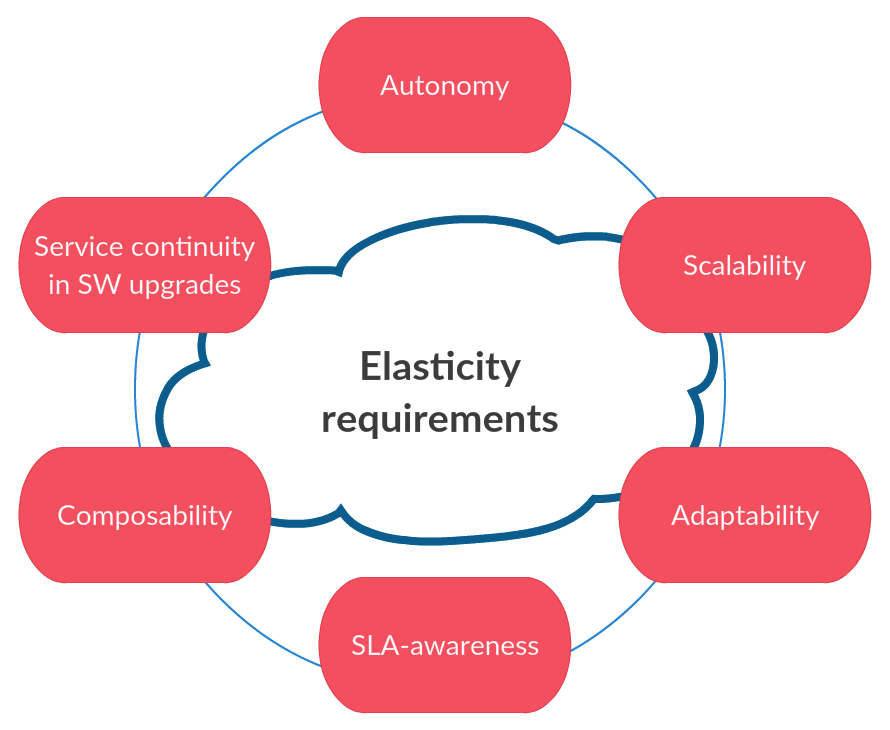
\includegraphics[scale=0.14]{images/elasticity-requirements.png}
				\end{figure}
			\end{column}
		\end{columns}
	}
	\only<2>
	{
		\begin{columns}
			\begin{column}{0.6\textwidth}
				Autonomy
				\begin{itemize}
					\item{\footnotesize{intelligent agent}}
					\item{\footnotesize{major-loop}}
					\begin{itemize}
						\item{\scriptsize{read from sensors $\rightarrow{}$ monitor}}
						\item{\scriptsize{read data || knowledge base $\rightarrow{}$ analyse}}
						\item{\scriptsize{plan actions $\rightarrow{}$ plan}}
						\item{\scriptsize{execute the plan $\rightarrow{}$ execute}}
					\end{itemize}
				\end{itemize}
			\end{column}
			\begin{column}{0.4\textwidth}
				\begin{figure}
					\centering{}
				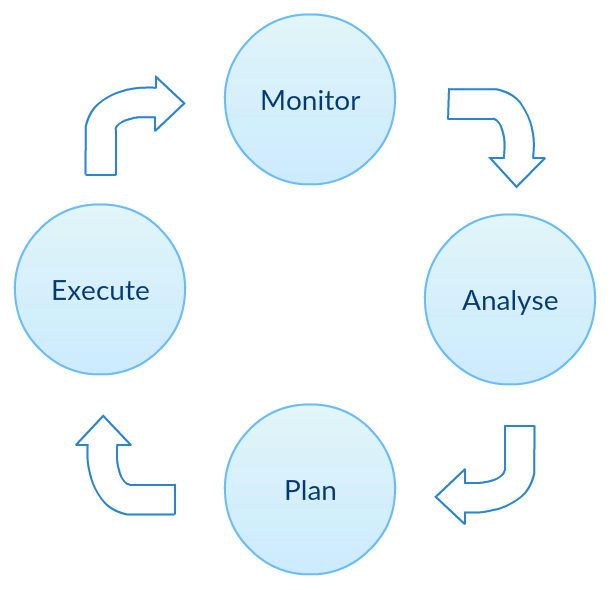
\includegraphics[scale=0.2]{images/autonomy.png}
				\end{figure}
			\end{column}
		\end{columns}
	}
	\only<3>
	{
		\begin{columns}
			\begin{column}{0.65\textwidth}
				Scalability:
				\begin{itemize}
					\item{\footnotesize{\textbf{replication (horizontal)}}}
					\begin{itemize}
						\item{\scriptsize{the only possible solution in PaaS}}
					\end{itemize}
					\item{\footnotesize{replicate some components when necessary}}
					\begin{itemize}
						\item{\scriptsize{the process must be transparent}}
						\item{\scriptsize{services must be well-designed}}
						\item{\scriptsize{classic architecture does not help}}
					\end{itemize}
					\item{\footnotesize{other: redimension (vertical) and migration}}
				\end{itemize}
			\end{column}
			\begin{column}{0.35\textwidth}
				\begin{figure}
					\centering{}
					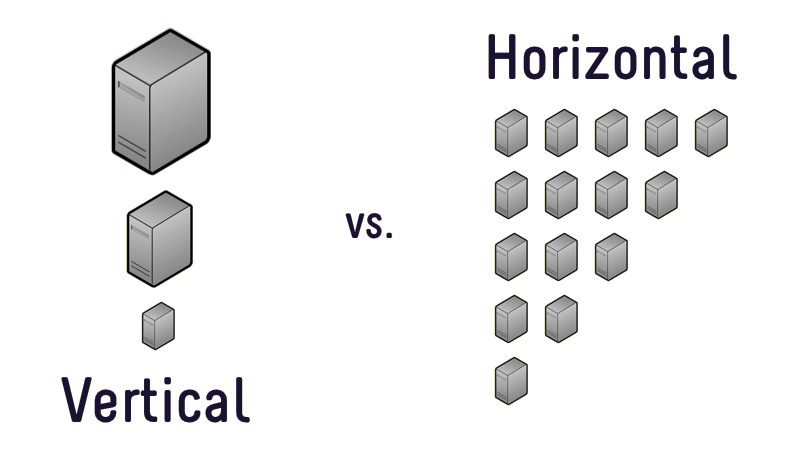
\includegraphics[scale=0.14]{images/scalability.png}
				\end{figure}
				\begin{flushright}
					\tiny{source: \url{https://goo.gl/orFWSi}}
				\end{flushright}
			\end{column}
		\end{columns}
	}
	\only<4>
	{
		\begin{columns}
			\begin{column}{0.6\textwidth}
				Adaptability dimensions
				\begin{itemize}
					\item{\footnotesize{adaptability}}
					\begin{itemize}
						\item{\scriptsize{services have to be designed to change at run-time}}
						\item{\scriptsize{automatic changes}}
					\end{itemize}
					\item{\footnotesize{adaptivity}}
					\begin{itemize}
						\item{\scriptsize{reactive}}
						\item{\scriptsize{proactive}}
						\item{\scriptsize{predictive $\rightarrow{}$ open research field}}
					\end{itemize}
				\end{itemize}
			\end{column}
			\begin{column}{0.4\textwidth}
				\begin{figure}
					\centering{}
					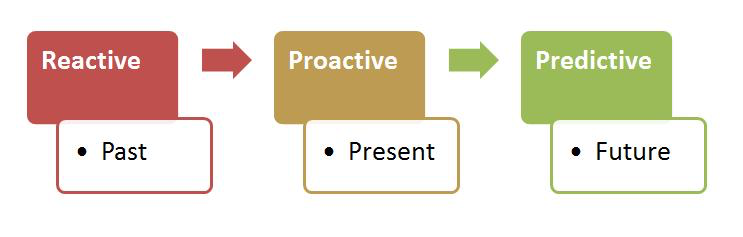
\includegraphics[scale=0.18]{images/adaptability.png}
				\end{figure}
				\begin{flushright}
					\tiny{source: \url{https://goo.gl/xv8Se6}}
				\end{flushright}
			\end{column}
		\end{columns}
	}
	\only<5>
	{
		\begin{columns}
			\begin{column}{0.55\textwidth}
				SLA-awareness
				\begin{itemize}
					\item{\footnotesize{consider customers needs}}
					\item{\footnotesize{QoS aspects}}
					\item{\footnotesize{\textbf{rich set of objectives}}}
				\end{itemize}
			\end{column}
			\begin{column}{0.45\textwidth}
				\begin{figure}
					\centering{}
					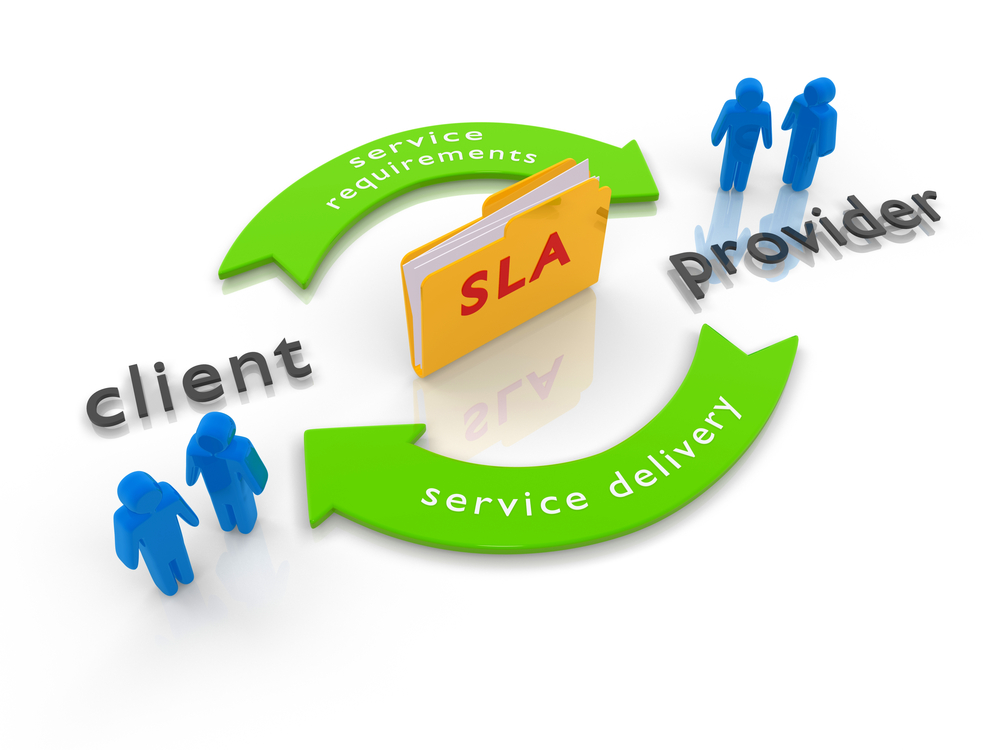
\includegraphics[scale=0.6]{images/sla.png}
				\end{figure}
				\begin{flushright}
					\tiny{source: \url{http://goo.gl/MW3VJm}}
				\end{flushright}
			\end{column}
		\end{columns}
	}
	\only<6>
	{
		\begin{figure}
			\centering{}
			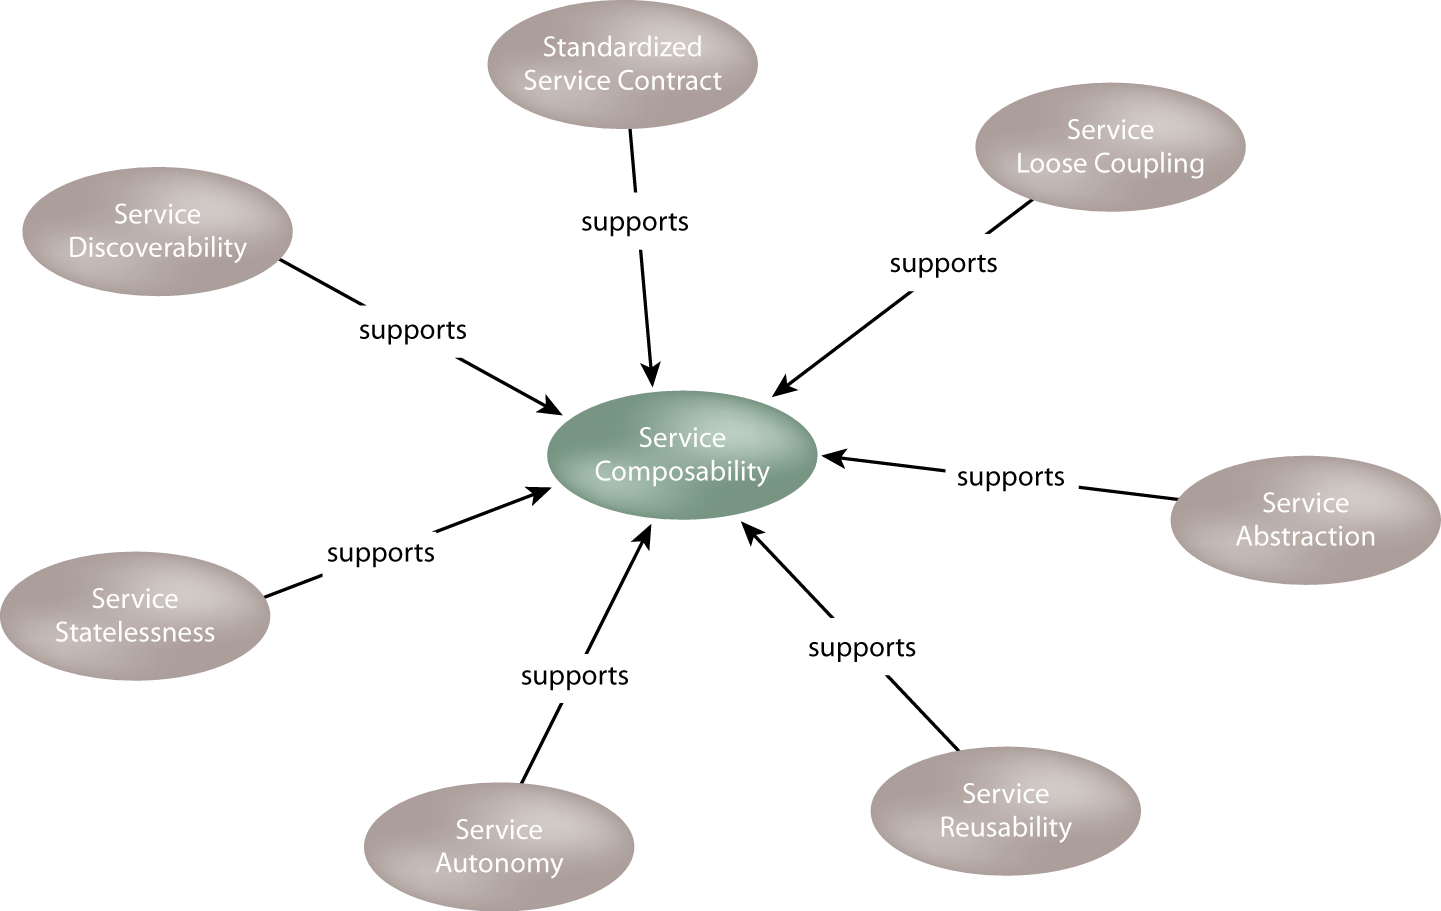
\includegraphics[scale=0.7]{images/composability.png}	
		\end{figure}
		\begin{flushright}
			\tiny{source: \url{http://goo.gl/2bpnfE}}
		\end{flushright}
	}
	\only<7>
	{
		\begin{columns}
			\begin{column}{0.55\textwidth}
				Service continuity in SW upgrades
				\begin{itemize}
					\item{\footnotesize{global consistency}}
					\item{\footnotesize{service availability}}
					\item{\footnotesize{coexistence and service continuity}}
					\item{\footnotesize{state transfer}}
					\item{\footnotesize{minimal overhead}}
				\end{itemize}
			\end{column}
			\begin{column}{0.45\textwidth}
				\begin{figure}
					\centering{}
					
\includegraphics[scale=0.5, angle=10]{images/upgrade.png}
				\end{figure}
				\begin{flushright}
					\tiny{source: \url{http://goo.gl/IU3eKk}}
				\end{flushright}
			\end{column}
		\end{columns}
	}
\end{frame}

\subsection{Multi-tenancy}
\begin{frame}{Multi-tenancy}
	\only<1>
	{
		\begin{columns}
			\begin{column}{0.6\textwidth}
				Requirements
				\begin{itemize}
					\item{\footnotesize{availability $\rightarrow{}$ redundant services}}
					\item{\footnotesize{secure tenants isolation}}
					\item{\footnotesize{guarantee of service $\rightarrow$ performance guarantee}}
					\item{\footnotesize{management of underlying resources}}
				\end{itemize}
				\begin{center}
					Software houses have to plan SLA with a rich set of \textbf{objectives}
				\end{center}
			\end{column}
			\begin{column}{0.4\textwidth}
				\begin{figure}
					\centering{}
					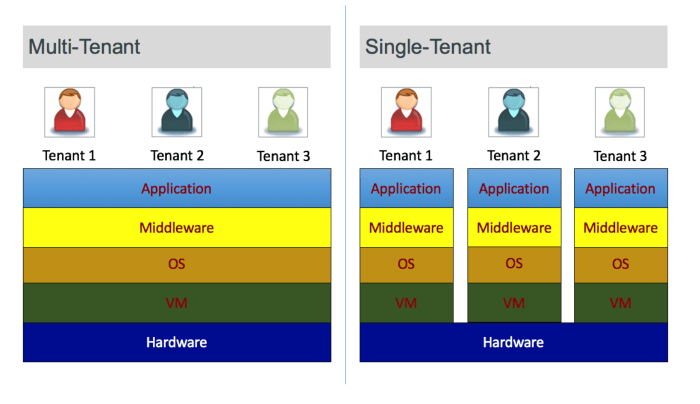
\includegraphics[scale=0.19]{images/multi-tenancy.png}
				\end{figure}
				\begin{flushright}
					\tiny{source: \url{http://goo.gl/MlsmWj}}
				\end{flushright}
			\end{column}
		\end{columns}
	}
	\only<2>
	{
		\begin{columns}
			\begin{column}{0.6\textwidth}
				Possible limits (\tiny{badly designed architecture}\normalsize{)}
				\begin{itemize}
					\item{\footnotesize{inflexibility}}
					\item{\footnotesize{security lack}}
					\item{\footnotesize{usability}}
					\begin{itemize}
						\item{\scriptsize{have to resist to high workload $\rightarrow{}$ elasticity}}
					\end{itemize}
					\item{\footnotesize{code rewriting}}
					\begin{itemize}
						\item{\scriptsize{high investments}}
					\end{itemize}
				\end{itemize}
			\end{column}
			\begin{column}{0.4\textwidth}
				\begin{figure}
					\centering{}
					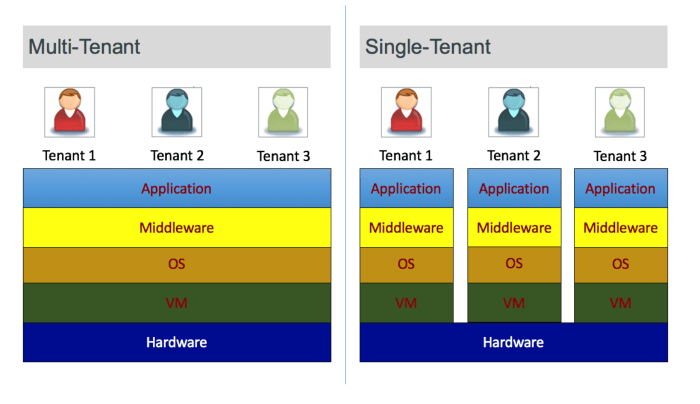
\includegraphics[scale=0.19]{images/multi-tenancy.png}
				\end{figure}
				\begin{flushright}
					\tiny{source: \url{http://goo.gl/MlsmWj}}
				\end{flushright}
			\end{column}
		\end{columns}
	}
\end{frame}